\chapter{算法实现}
本章,我们将从判决预测、关键词抽取、类案搜索等模块来详细介绍项目中用到的算法模型。在模型中,我们统一使用了THULAC进行中文分词,我们使用的词向量是利用FastText模型,在大规模的法律文书语料库上进行的预训练,我们采用的词向量维度为200维。

对于每一个模块,我们将分别从任务的描述定义、算法的创新点、算法模型细节三个方面来进行详细阐述。

\section{背景知识}
\subsection{卷积神经网络}
卷积神经网络(Convolutional Neural Network, CNN)是一种前馈神经网络,它的人工神经元可以响应一部分覆盖范围内的周围单元,对于大型图像、文字等处理有出色表现。

卷积神经网络通常包含以下结构:

\begin{itemize}
	\item \textbf{卷积层(Convolutional layer)}:卷积神经网路中每层卷积层由若干卷积单元组成,每个卷积单元的参数都是经过\textbf{反向传播算法}训练得到的。卷积运算的目的是提取输入的不同特征。
	\item \textbf{线性整流层(Rectified Linear Units layer, ReLU layer)}:使用线性整流作为激活函数。它可以增强判定函数和整个神经网络的非线性特性,而本身并不会改变卷积层。
	\item \textbf{池化层(Pooling layer)}:通常在卷积层之后会得到维度很大的特征,将特征切成几个区域,取其最大值或平均值,得到新的、维度较小的特征。
	\item \textbf{全连接层(Fully-Connected layer)}:完成从输入到标签集的映射,即分类。
\end{itemize}

\begin{figure*}[h]
    \centering
    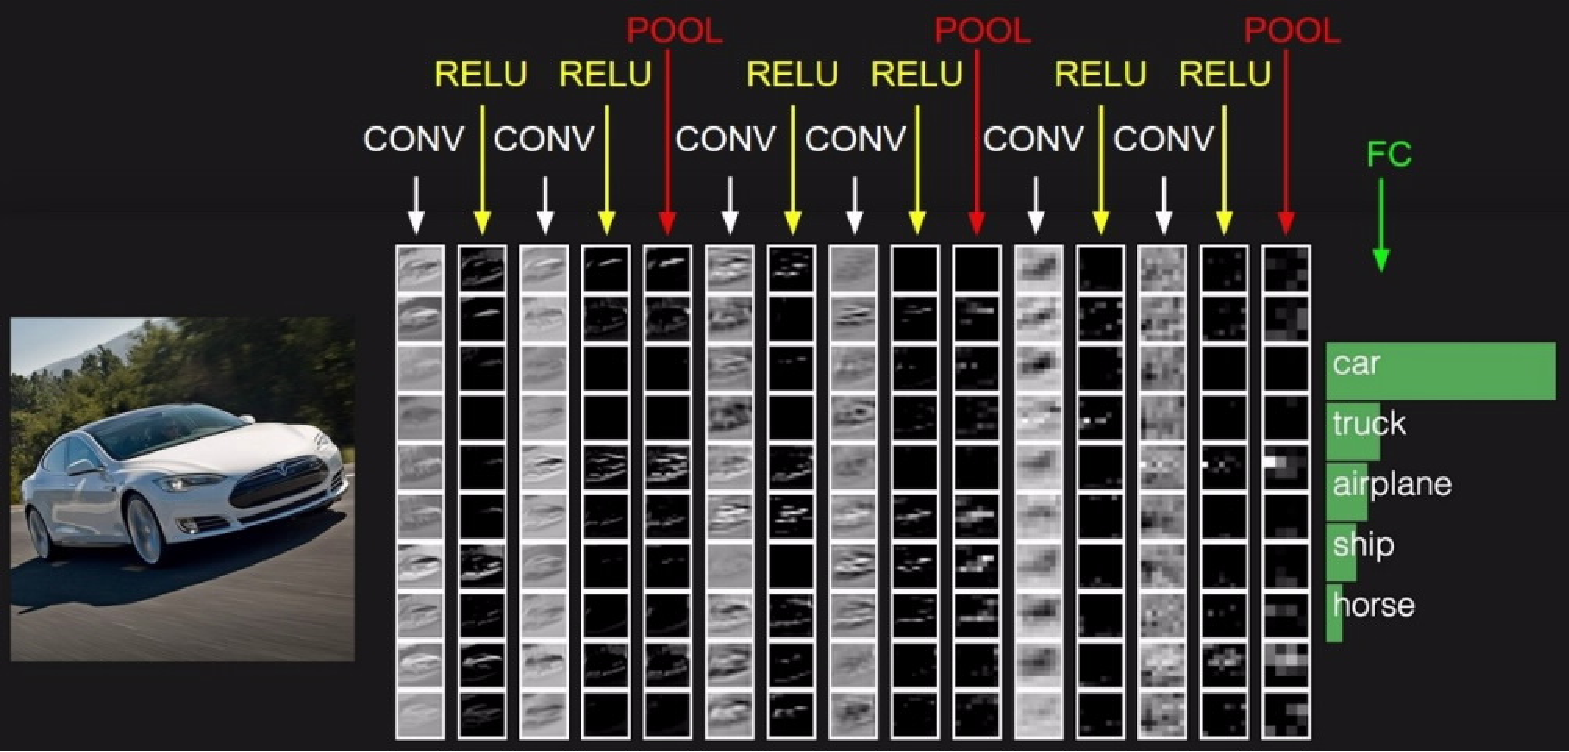
\includegraphics[width=\linewidth]{figures/cnn1}
    \caption{卷积神经网络实例}
    \label{fig:cnn1}
\end{figure*}

图~\ref{fig:cnn1}是一个卷积神经网络各层应用的实例:


卷积神经网络中最基础的操作是卷积。基础 CNN 所用的卷积是一种 2-D 卷积。也就是说,卷积核(kernal)只能在 x,y 上滑动位移,不能进行深度(跨通道)位移。

卷积需要输入两个参数,实质是二维空间滤波,滤波的性质与卷积核选择有关,CNN 的卷积是在一个 2-D 卷积核与 2-D 输入映射之间,在各通道分别完成的。

我们假设单一通道输入的空间坐标为 ${\displaystyle (x,y)}$,kernel 大小是 ${\displaystyle p \times q}$,kernel 权重为 ${\displaystyle w}$,图像亮度值是 ${\displaystyle v}$,卷积过程就是 kernel 所有权重与其在输入图像上对应元素亮度之和,可以表示为:${\displaystyle conv_{x,y} = \sum_i^{p*q}w_i v_i}$。

下面即是一个例子:

\begin{figure*}[ht]
    \centering
    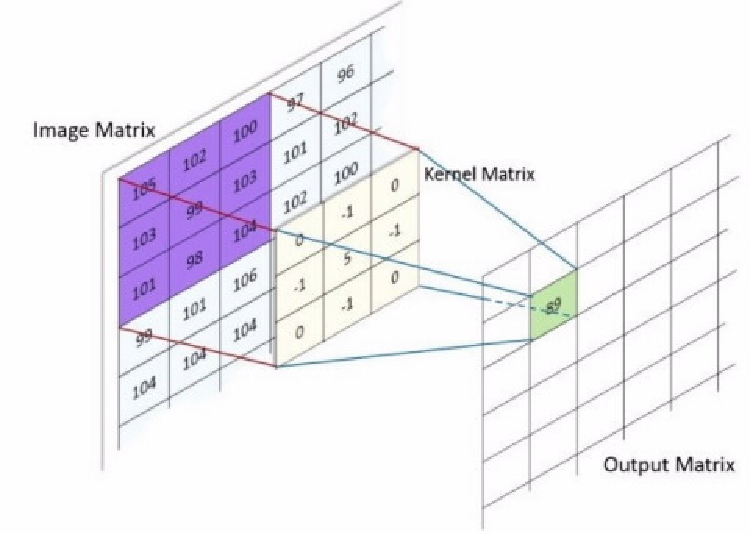
\includegraphics[width=\linewidth]{figures/cnn_conv}
    \caption{卷积层的例子}
    \label{fig:cnn_conv}
\end{figure*}

将 kernel 随 ${\displaystyle (x,y)}$ 平移扫描,即可以得到输出空间。需要特别说明的是,卷积层可能包含多个 kernel,用以抓取多个特征;扫描步长、方向也可能有所不同。

卷积之后,通常会加入偏置(bias),并引入非线性激活函数(activation function),令偏置为 ${\displaystyle b}$,激活函数为 ${\displaystyle h\left(\right)}$,经过激活函数后,得到的结果是 ${\displaystyle z_{x,y}=h\left(\sum_i^{p*q} w_i v_i +b\right)}$。

池化(Pooling)是卷积神经网络中另一个重要的概念,它实际上是一种形式的降采样。有多种不同形式的非线性池化函数,而其中“最大池化(Max pooling)”是最为常见的。它是将输入的图像划分为若干个矩形区域,对每个子区域输出最大值。直觉上,这种机制能够有效地原因在于,在发现一个特征之后,它的精确位置远不及它和其他特征的相对位置的关系重要。池化层会不断地减小数据的空间大小,因此参数的数量和计算量也会下降,这在一定程度上也控制了过拟合。通常来说,CNN 的卷积层之间都会周期性地插入池化层。

池化层通常会分别作用于每个输入的特征并减小其大小。目前最常用形式的池化层是每隔 2 个元素从图像划分出 ${\displaystyle 2\times 2}$ 的区块,然后对每个区块中的 4 个数取最大值。这将会减少 75% 的数据量。

出现在 CNN 最后的全连接层的主要目的是分类。这与神经网络中的全连接层是相同的。

CNN 网络的训练一般使用反向传播(Back Propagation)算法。同样地,这即是传统神经网络训练的常用算法。


\subsection{长短时记忆网络}

长短时记忆网络(Long short-term memory, LSTM)是一种用于深度学习领域的循环神经网络(Recurrent Neural Network, RNN)架构。与其他神经网络架构不同,LSTM 网络非常适合基于时间序列数据进行分类、处理和预测。

循环神经网络相比全连接神经网络更擅长处理序列数据,与传统神经网络不同,它们是具有循环的网络,这将允许信息持续存在。

咕咕咕,这里有一张图

上图是一个示意图,一组神经网络 A 接收某些输入 ${\displaystyle x_t}$,并输出一个值 ${\displaystyle h_t}$。循环允许信息从网络的一个步骤传递到下一个。

RNN 的重要能力在于它可以将以前的信息连接到当前任务,例如使用先前的视频帧来帮助对当前帧的理解。然而,对于较长距离的历史信息,RNN 仍无法有效地将其利用。

LSTM 相对 RNN 而言解决了长依赖关系学习的问题,能够记住长时间间隔内的信息。通常地,一个 LSTM 单元包含细胞、输入门、输出门和忘记门。其中,细胞(用${\displaystyle C_t}$ 表示)用于记录需要的长时间间隔的信息;输入门、输出门、忘记门具有删除或添加信息到细胞状态的能力,它们被用于维护细胞的状态、控制进出单元的信息流。

下图是一个示意图:

咕咕咕,这里有另一张图




\subsection{条件随机场}


\section{判决预测}
\subsection{任务描述}
在该模块中,我们主要实现了案件的罪名及案由预测、相关法条推荐、刑事案件刑期预测、相关判案要素预测等功能。

输入一段文本形式的案情描述,模型通过阅读文本获取文本中蕴含的语义信息,将案情映射到一个高维向量空间中,得到一个包含有文本信息的文章向量,再根据不同的任务,将文章向量喂给不同的输出层获得不同的分类结果。

\subsection{创新点}
我们将上述所有功能归纳为文本分类问题,通过观察,上述任务之间有很强的前后依赖关系,例如,相关法条推荐结果往往与罪名及案由预测结果高度相关。并且,根据法学领域从业人员介绍,在实际判案时,大家首先会判断案情中的相关要素,并根据要素判断结果来决定最后的案件的判决。因此,我们有以下创新来提升各个任务的效果:

1)	在多任务学习(multi-task learning)中提出了一个新的架构,充分利用各个任务之间的依赖关系来共同提升多个任务的预测效果。

2)	模拟法官判案过程,提出判断案件判案要素作为中间任务,来大幅提升相关任务的效果。



\subsection{算法模型}
算法使用了LSTM作为模型的编码器,使用了全连接神经网络作为输出层。利用了多任务学习的框架,将多个任务进行联合训练得到了效果的提升。

我们在获得案情文本后,可将算法分为以下几步:
\begin{itemize}
	\item \textbf{输入层}:文本分词与词向量映射。通过上文提到的THULAC与FastText完成本步,将文章映射成词向量序列。
	\item \textbf{编码层}:我们利用了LSTM循环神经网络对词向量序列进行编码,得到一个隐向量序列。之后,我们利用了self-attention机制,来获得对应于不同任务的文本信息。
	\item \textbf{预测层}:我们利用了LSTM Cell来捕获不同任务之间的依赖关系,将不同的任务获得的文本向量当做一个序列,使得任务之间可以获取相应被依赖任务的信息,从而提升相应的效果。
	\item \textbf{输出层}:最后,我们应用了全连接神经网络,将包含任务信息的向量映射到相应的分类中。
\end{itemize}

\begin{figure*}[ht]
    \centering
    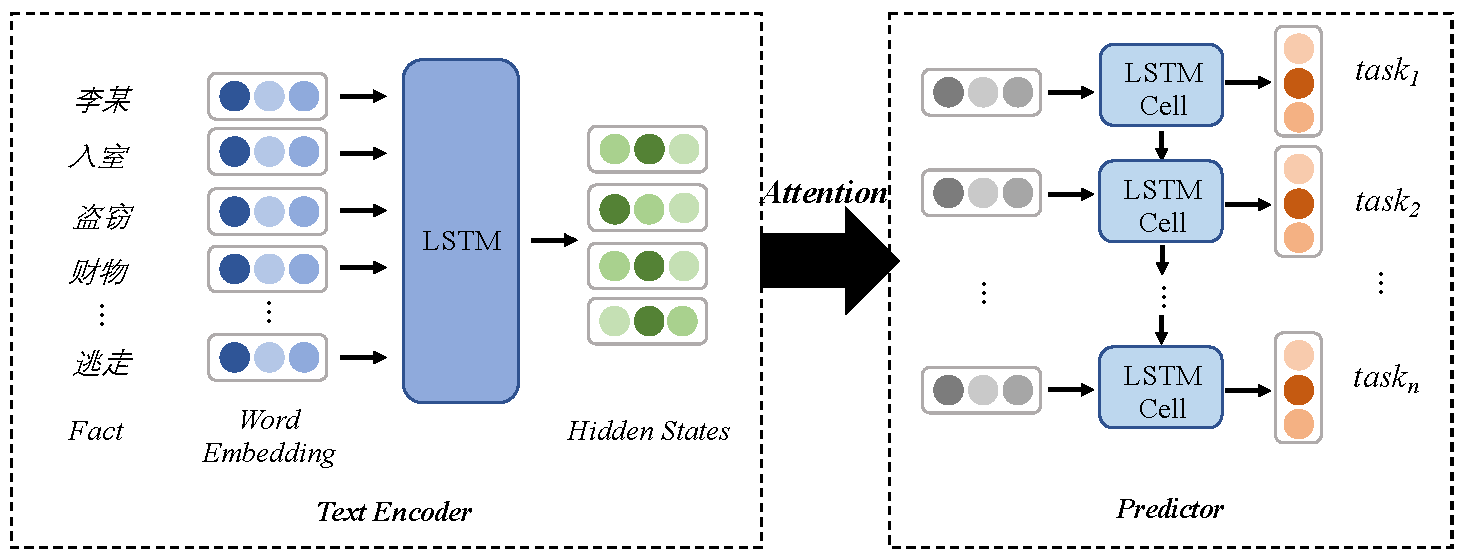
\includegraphics[width=\linewidth]{figures/model1}
    \caption{判决预测模型示意图}
    \label{fig:model1}
\end{figure*}


\section{关键词抽取}
\subsection{任务描述}
在该模块中,我们利用了序列标注模型实现了对案情文本的关键词抽取。任务输入仍旧为一段案情描述的文本,任务的输出为文本中的某一个或者某一些词语,这些词语与法律词汇高度相关,是用来检索相关案件、法条的重要依据。

例如,对于句子:“被告对{\color{red}火灾}发生是否存在{\color{red}过错},应否对原告的合理损失予以{\color{red}赔偿}”中标红的即为关键词,对于检索相关法律法规:“关于{\color{red}火灾过错}引发事故责任划分与{\color{red}赔偿}…”有很强的指导意义。

本模块我们采用了对句子级别的预料进行训练的方式,我们整理了10000条待标注数据,通过寻找专业人士进行人工标注的方法,获取了相应的待标注的训练数据。

在使用时,我们将对每一个句子进行关键词抽取,通过算法规则将所有句子的关键词进行合并、筛选,得到最终文章级别的关键词。关键词抽取的结果将对后续的相关案例检索提供重要的帮助。

\subsection{创新点}

关键词抽取是自然语言处理中,非常常见的任务。在早期,大多数人们使用的是基于词频等特征的无监督学习算法,例如TextRank、LDA、TFIDF算法。对于法律这样一个特定领域,关键词抽取的结果往往是一些法言法语,相比于开放领域上的关键词抽取,有着更强的规律性。因此,我们将目前效果最好的命名实体识别算法运用至该任务。同时,由于训练是在句子级别的语料上进行训练,我们设计了筛选算法,将在所有句子上的抽取结果进行合并筛选,得到了一个较好的效果。

\subsection{算法模型}

\begin{figure*}[ht]
    \centering
    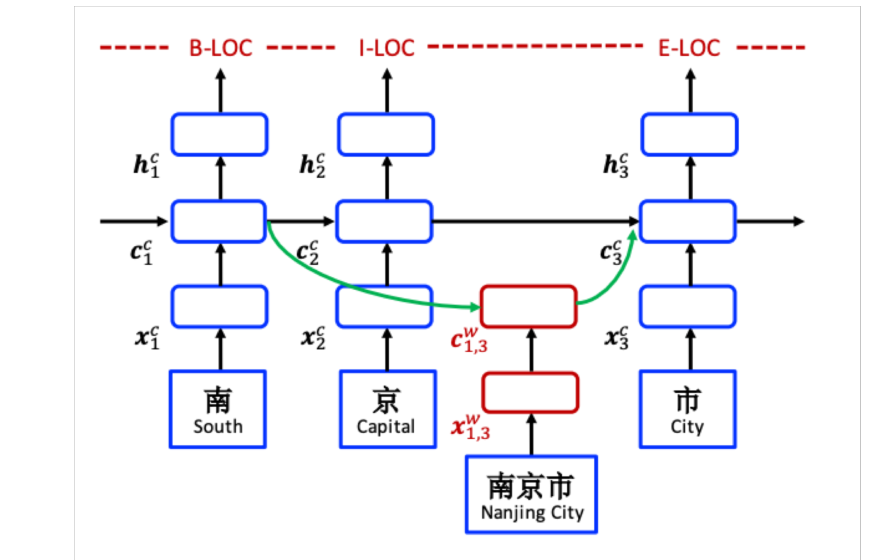
\includegraphics[width=\linewidth]{figures/model2}
    \caption{关键词抽取模型示意图}
    \label{fig:model2}
\end{figure*}

该算法将目前前沿的命名实体识别算法——Lattice LSTM,通过将句子拆分成字级别,对每一个字一个标签,来判断最终关键词的范围。在传统的基于字级别的模型基础上,加入词级别信息,这样克服了字级别信息不足、词级别过度依赖于分词效果的缺陷。

1)	利用n-gram、分词信息等特征为句子中每一个字进行编码,形成字级别特征;

2)	利用好BiLSTM-CRF的框架,通过BiLSTM对字特征进行编码,再通过CRF捕捉序列信息,进行序列标注;

3)	改造字级别的LSTM模型,将字与字之间匹配成的所有的可能词的特征融合到LSTM的信息传递中,得到一个Lattice-word model;

4)	对每个字预测BIE标签,其中B为begin、I为in、E为end;得到最后序列标注的结果。



\section{类案搜索}
\subsection{任务描述}
该模块实现了相关案例推荐的功能。该功能的实现主要基于上述两个模块的模型。该任务模型以案情描述作为输入,通过关键词标签抽取,检索到一批与该案情相似的法律文书,再利用判决预测模块得到的文本向量,对检索到的文书进行重排序,输出一个按照相似度递减的法律文书集合。

\subsection{创新点}
该任务所用算法与传统的搜索引擎算法不同,传统搜索引擎将检索文本与数据库文本进行比对,进而检索出相似度高的文本段。在我们算法中,我们通过抽取出的关键词标签来初步确定相关的文章的集合,再通过判决预测模块中获得的包含文本语义的向量,来对相关集合进行重排序,得到在语义层面相似度最高的文章。

这样的做法改善了传统搜索引擎只关注文本相似度的缺点,通过捕捉语义信息检索以满足用户需求。

\subsection{算法模型}
如上所述,改算法主要分成以下两步:

1)	抽取关键词,利用关键词抽取模块将案情描述中的关键词抽取出来。

2)	利用关键词标签,确定相关文书的集合;将所有关键词与该案情描述关键词一样的案件抽取出来,形成相关文书集合。

3)	相关程度重排序,利用判决预测模块将第2步获得的文书,转化成包含语义信息的文本向量,通过向量的距离来判断文书与输入案情的相关程度,按照相关程度对文书进行重排序。



